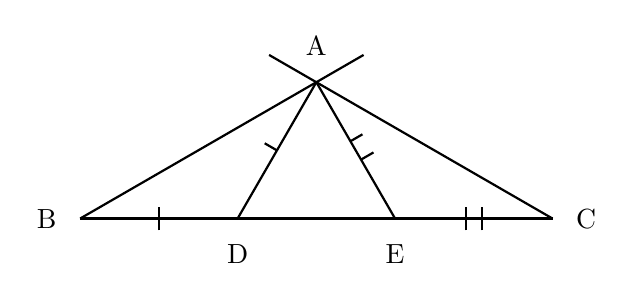
\begin{tikzpicture}[scale=1]

    % --- Coordinates ---
    % Base line points: B(0,0), D(2,0), E(4,0), C(6,0)
    \coordinate (B) at (0,0);
    \coordinate (D) at (2,0);
    \coordinate (E) at (4,0);
    \coordinate (C) at (6,0);
    
    % Vertex A calculated for isosceles properties BD=AD and AE=EC
    \coordinate (A) at (3,1.732);

    % --- Main Geometric Lines ---
    \draw[thick] (B) -- (C); % Base line BC
    \draw[thick] (A) -- (D); % Internal segment AD
    \draw[thick] (A) -- (E); % Internal segment AE

    % --- Vertex A Crossing ---
    % AB and AC lines extend past A to replicate the intersection
    \draw[thick] (B) -- (3.6, 2.078); 
    \draw[thick] (C) -- (2.4, 2.078);

    % --- Balanced Tick Marks ---
    
    % 1. Single vertical tick on segment BD
    \draw[thick] (1, -0.15) -- (1, 0.15);
    
    % 2. Single perpendicular tick on segment AD
    \draw[thick] (2.5, 0.866) + (150:0.18) -- (2.5, 0.866) + (-30:0.18);

    % 3. ACCURATE DOUBLE perpendicular ticks on segment AE
    % Spacing reduced to 0.15 units for a balanced look
    \draw[thick] (3.43, 0.98) + (30:0.18) -- (3.43, 0.98) + (210:0.18); % Tick 1
    \draw[thick] (3.57, 0.75) + (30:0.18) -- (3.57, 0.75) + (210:0.18); % Tick 2

    % 4. ACCURATE DOUBLE vertical ticks on segment EC
    % Spaced at 4.9 and 5.1
    \draw[thick] (4.9, -0.15) -- (4.9, 0.15);
    \draw[thick] (5.1, -0.15) -- (5.1, 0.15);

    % --- Point Labels ---
    % Positioned exactly as shown in Figure 7
    \node[above=6pt] at (A) {A};
    \node[left=5pt] at (B) {B};
    \node[right=5pt] at (C) {C};
    \node[below=6pt] at (D) {D};
    \node[below=6pt] at (E) {E};

\end{tikzpicture}